\section{The System}
This section will give a general overview of the system. 
A block diagram of the system is presented, see figure \ref{fig:block}, and each block will be given a brief explanation.
Each subsequent section will seek to explain the purpose and functionality of a block in more detail.\\~\\

\begin{figure}[H]
	\centering
	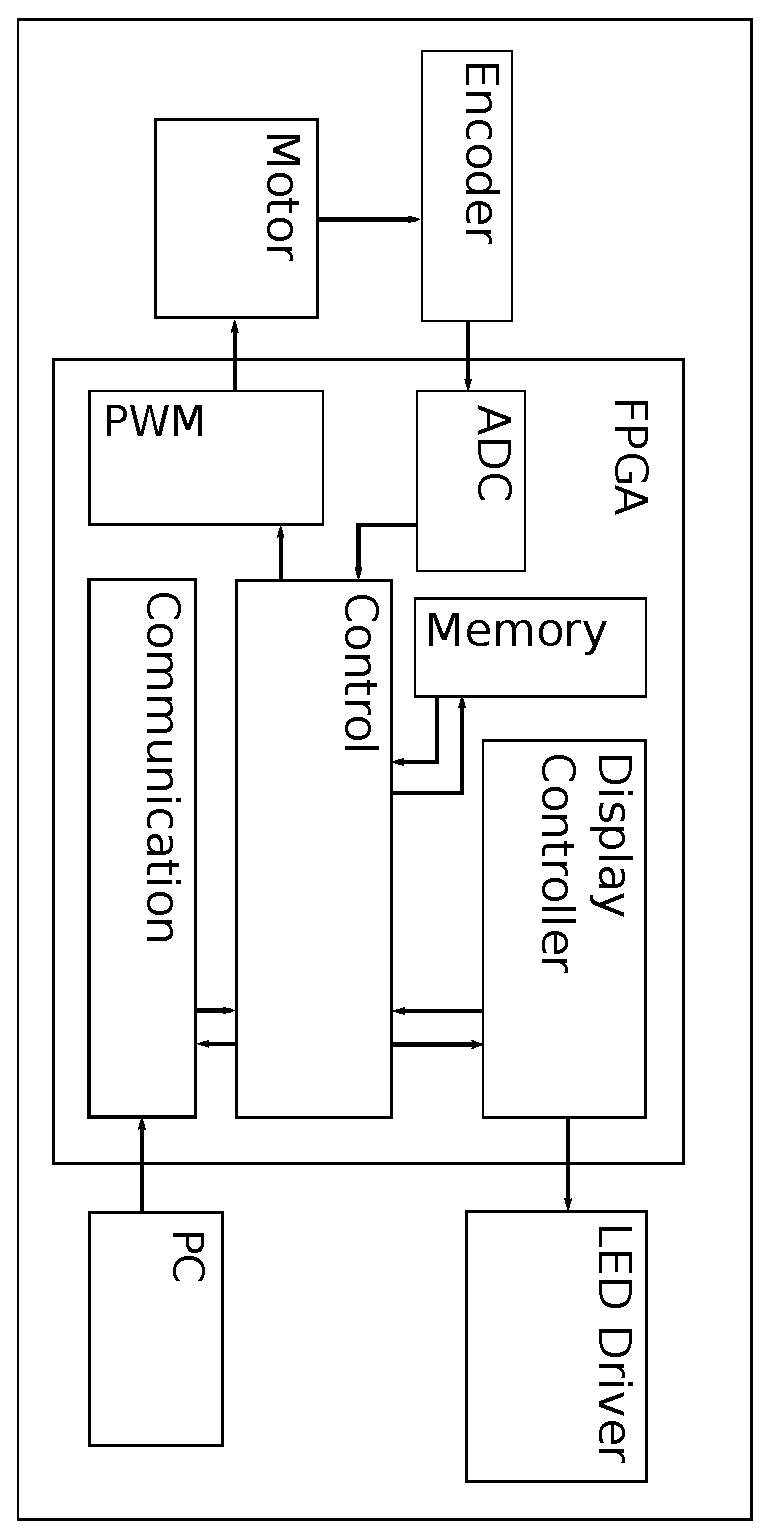
\includegraphics[angle=90,width=.8\linewidth]{images/block_diagram}
	\caption{Block diagram of the rotating LED display.}
	\label{fig:block}
\end{figure}

The display is rotated using a PWM controlled DC motor.
Due to the excessive capabilities of the motor, a gearing is developed to limit its rotational speed.
In order to stably show an image it is necessary to keep the rotational speed of the motor reasonably constant.
This is done by adding an encoder to the motor.
The output of the encoder is then used to set the duty cycle of the PWM to a suitable value.

Due to the limited memory available on the FPGA, only one image is stored locally at any one time.
Any subsequent images will be transmitted to the FPGA from a PC using $\mu$TosNet.
A display controller is written in VHDL.
It is the task of this controller to send the correct instructions to the LED driver, such that the correct pixels are displayed in the correct order.

Finally, a general control block is written.
This block will act as the interface between all of the components present on the FPGA.
